\documentclass[12pt]{article}
\usepackage[english]{babel}
\usepackage[utf8x]{inputenc}
%\usepackage[a4paper, total={6in, 8in}]{geometry}
\usepackage[margin=0.5in]{geometry}
\usepackage{graphicx}
\usepackage{subcaption}
\usepackage{placeins}
\renewcommand{\thesubsection}{\thesection.\alph{subsection}}

%-------------- TITLE -----------------%
\author{James Ogle}
\title{ECE414 -- Milestone 3}

%---------- START DOCUMENT ------------%
\begin{document}
    \pagenumbering{gobble}
    \maketitle
    \pagenumbering{arabic}

    %-----------------------------------------%
    \section*{Project Progress}
    \begin{itemize}
        \item The focus during this section of the project has been focused developing the Q-learning algorithm for create a Q-table for the agent.
        After Q-learning was developed, the next part of the process of analyzing the results to confirm the agent was able to "learn" in the environment and improves its actions.
        \item No major changes have been made to the environment.
        The only change implemented into the environment was the viewable-space by the agent, changed from 5x5 to 3x3 grid space in front.
        \item The next focus will be implementing a way for the agent to operate consistently well on grids it has not seen before.
        Currently, it is able to learn and be 100\% accurate the grid it was trained on which does not mean anything for the real world.
    \end{itemize}

    %-----------------------------------------%
    \section*{RL Algorithm Implementation}
    \begin{itemize}
        \item \textbf{Algorithm:} Q-learning with linear epsilon decay is the algorithm implemented to train the agent.
        \item \textbf{Reason:} I chose Q-learning since it learns strictly from the policy.
        This means in ideal sense, it should aim for choosing the most optimal route.
        Since the environment I have setup does not have meaning hazards to account for, the potential of Q-learning causing rover to fail catastrophically in unseen grids seemed unlikely.
        However, in order to make sure the agent explores, I implemented linear decay so the agent would explore more in the earlier episodes and becoming more greedy in the later episodes.
        \item \textbf{Action Selection:} The agent uses an epsilon-greedy action-selection policy.
        With probability $\epsilon$, it selects one of the four movement actions randomly to explore the environment.
        Otherwise, it selects the action with the largest current Q-value for the observed state.
        During training, $\epsilon$ gradually decreases so the rover explores more at the beginning and relies more on learned actions later. 
        \item \textbf{Learning:}
            \[
            Q(s,a) \leftarrow Q(s,a) + \alpha \left[r + \gamma \max_{a'} Q(s',a') - Q(s,a)\right].
            \]
        Here, $\alpha$ is the learning rate and $\gamma$ is the discount factor.
        The algorithm directly updates Q-values rather than a separate policy table; the policy improves indirectly because the agent chooses the action with the highest Q-value in each state.
    \end{itemize}
    \begin{figure}[!ht]
        \centering
        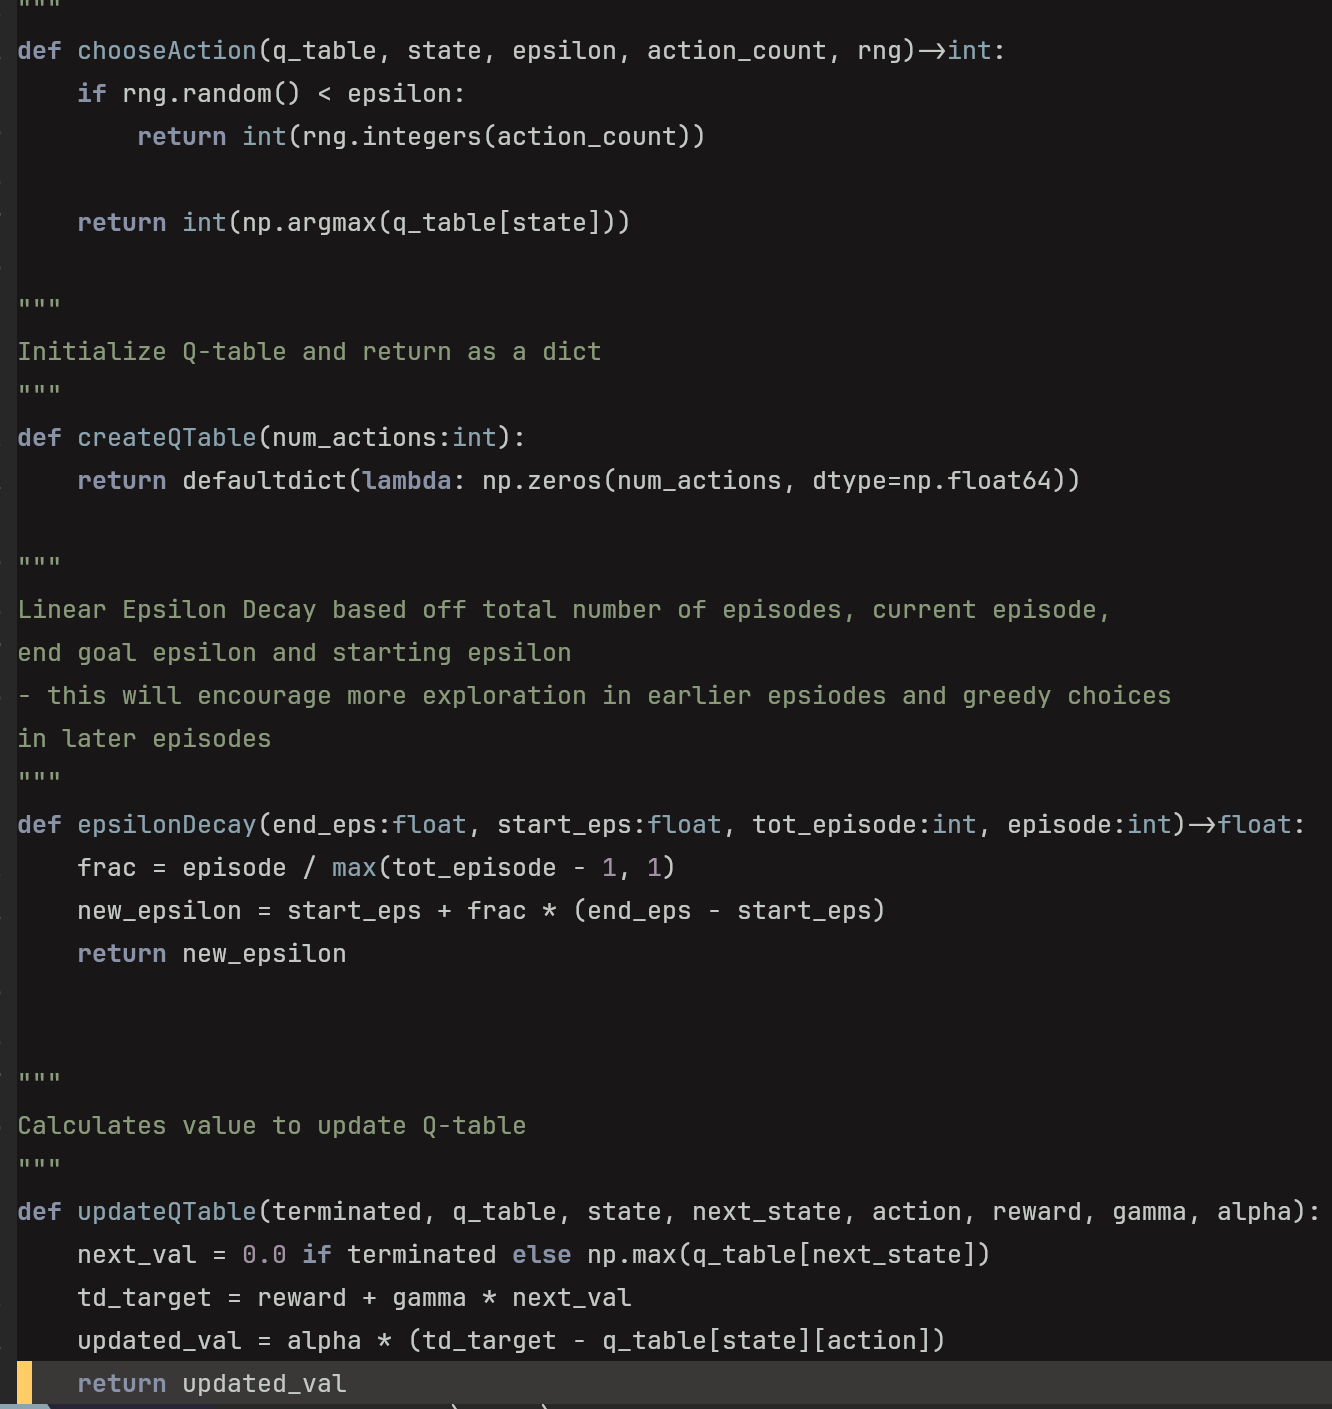
\includegraphics[scale=0.20]{./img/rl_algo.png}
        \caption{Code implementation for Reinforcement Learning Algorithm Q-learning}
    \end{figure}
    
    \FloatBarrier

    %-----------------------------------------%
    \section*{Training Process}
    \begin{itemize}
        \item Algorithm implemented for the training process is Q-learning with linear decay for the epsilon
        \item Parameters used for the algorithm are epsilon start and end, episodes (these 3 are for calculating epsilon decay), discount factor (gamma), and learning rate (alpha) 
        \item The agents Q-values are updated through: 
            \[
            Q(s,a) \leftarrow Q(s,a) + \alpha \left[r + \gamma \max_{a'} Q(s',a') - Q(s,a)\right].
            \]
    \end{itemize}
    \begin{figure}[!ht]
        \centering
        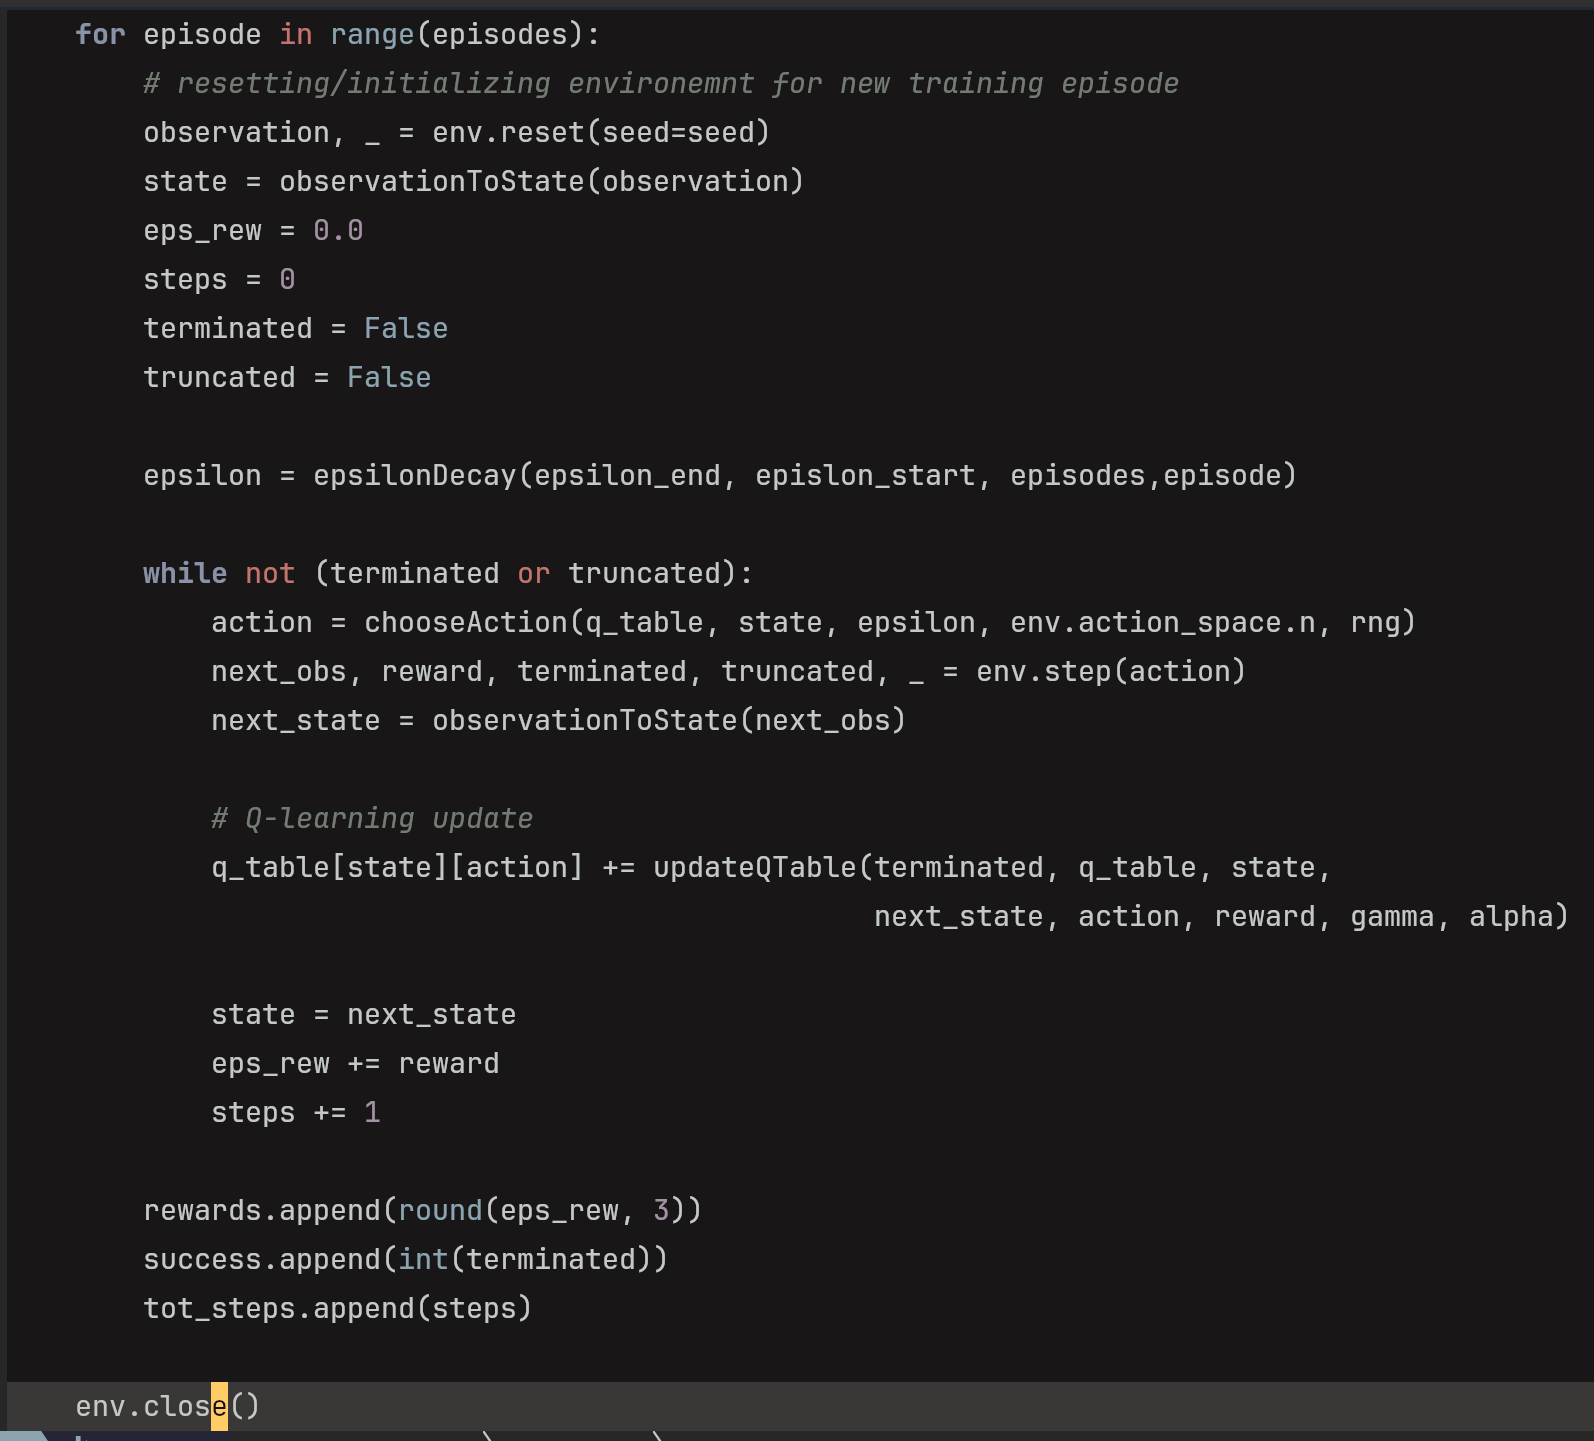
\includegraphics[scale=0.15]{./img/train_code.png}
        \caption{Code for training the RL agent}
    \end{figure}

    \FloatBarrier

    The rover is trained using tabular Q-learning, which updates Q-values that estimate the long-term reward of each action in a given state. At the start of each episode, the environment resets and provides the rover with an initial partial observation.
    The rover converts this observation into a state and uses an epsilon-greedy policy to select one of four movement actions.
    After each action, the environment returns the next observation, reward, and episode status, which the agent uses to update the Q-value for its previous state-action pair.
    In order to update the Q-value, the training process includes epsilon, learning rate, and discount factor into the Q-value update equation.
    This cycle continues until the rover reaches the goal or the episode reaches the maximum step limit. 

    %-----------------------------------------%
    \section*{Initial Results \& Baseline}
    \begin{itemize}
        \item The agent is able to achieve a reward value of 1.54 and 19 steps per an episode after training. However this is only when using the same grid for the evaluation.
        When the grid changes on each episode randomly, then the agent will fail or succeed at random.
        \item The agent is improving during training which can be seen in the graphs below where the rewards per episode increases as the number of episodes increases.
        This can also be seen in the steps as well where the number of steps is decreasing over time.
        The steps decreasing is one of the goals of the agent since it means it is taking less steps per an episode in order to find the goal (aka, it is finding a quicker path each time).
        \item Currently, the evaluation metrics being used to measure the agent's progress are the number of steps and total reward value per an episode.
        With the introduction of new environments for the agent each episode, I will introduce a success rate metric to capture how many successful runs it has.
        I found this metric not to be helpful currently since the agent has 100\% success rate during the evaluation but collapses to around 50\% when new grids are introduced.
    \end{itemize}
    \begin{figure}[!ht]
        \centering
        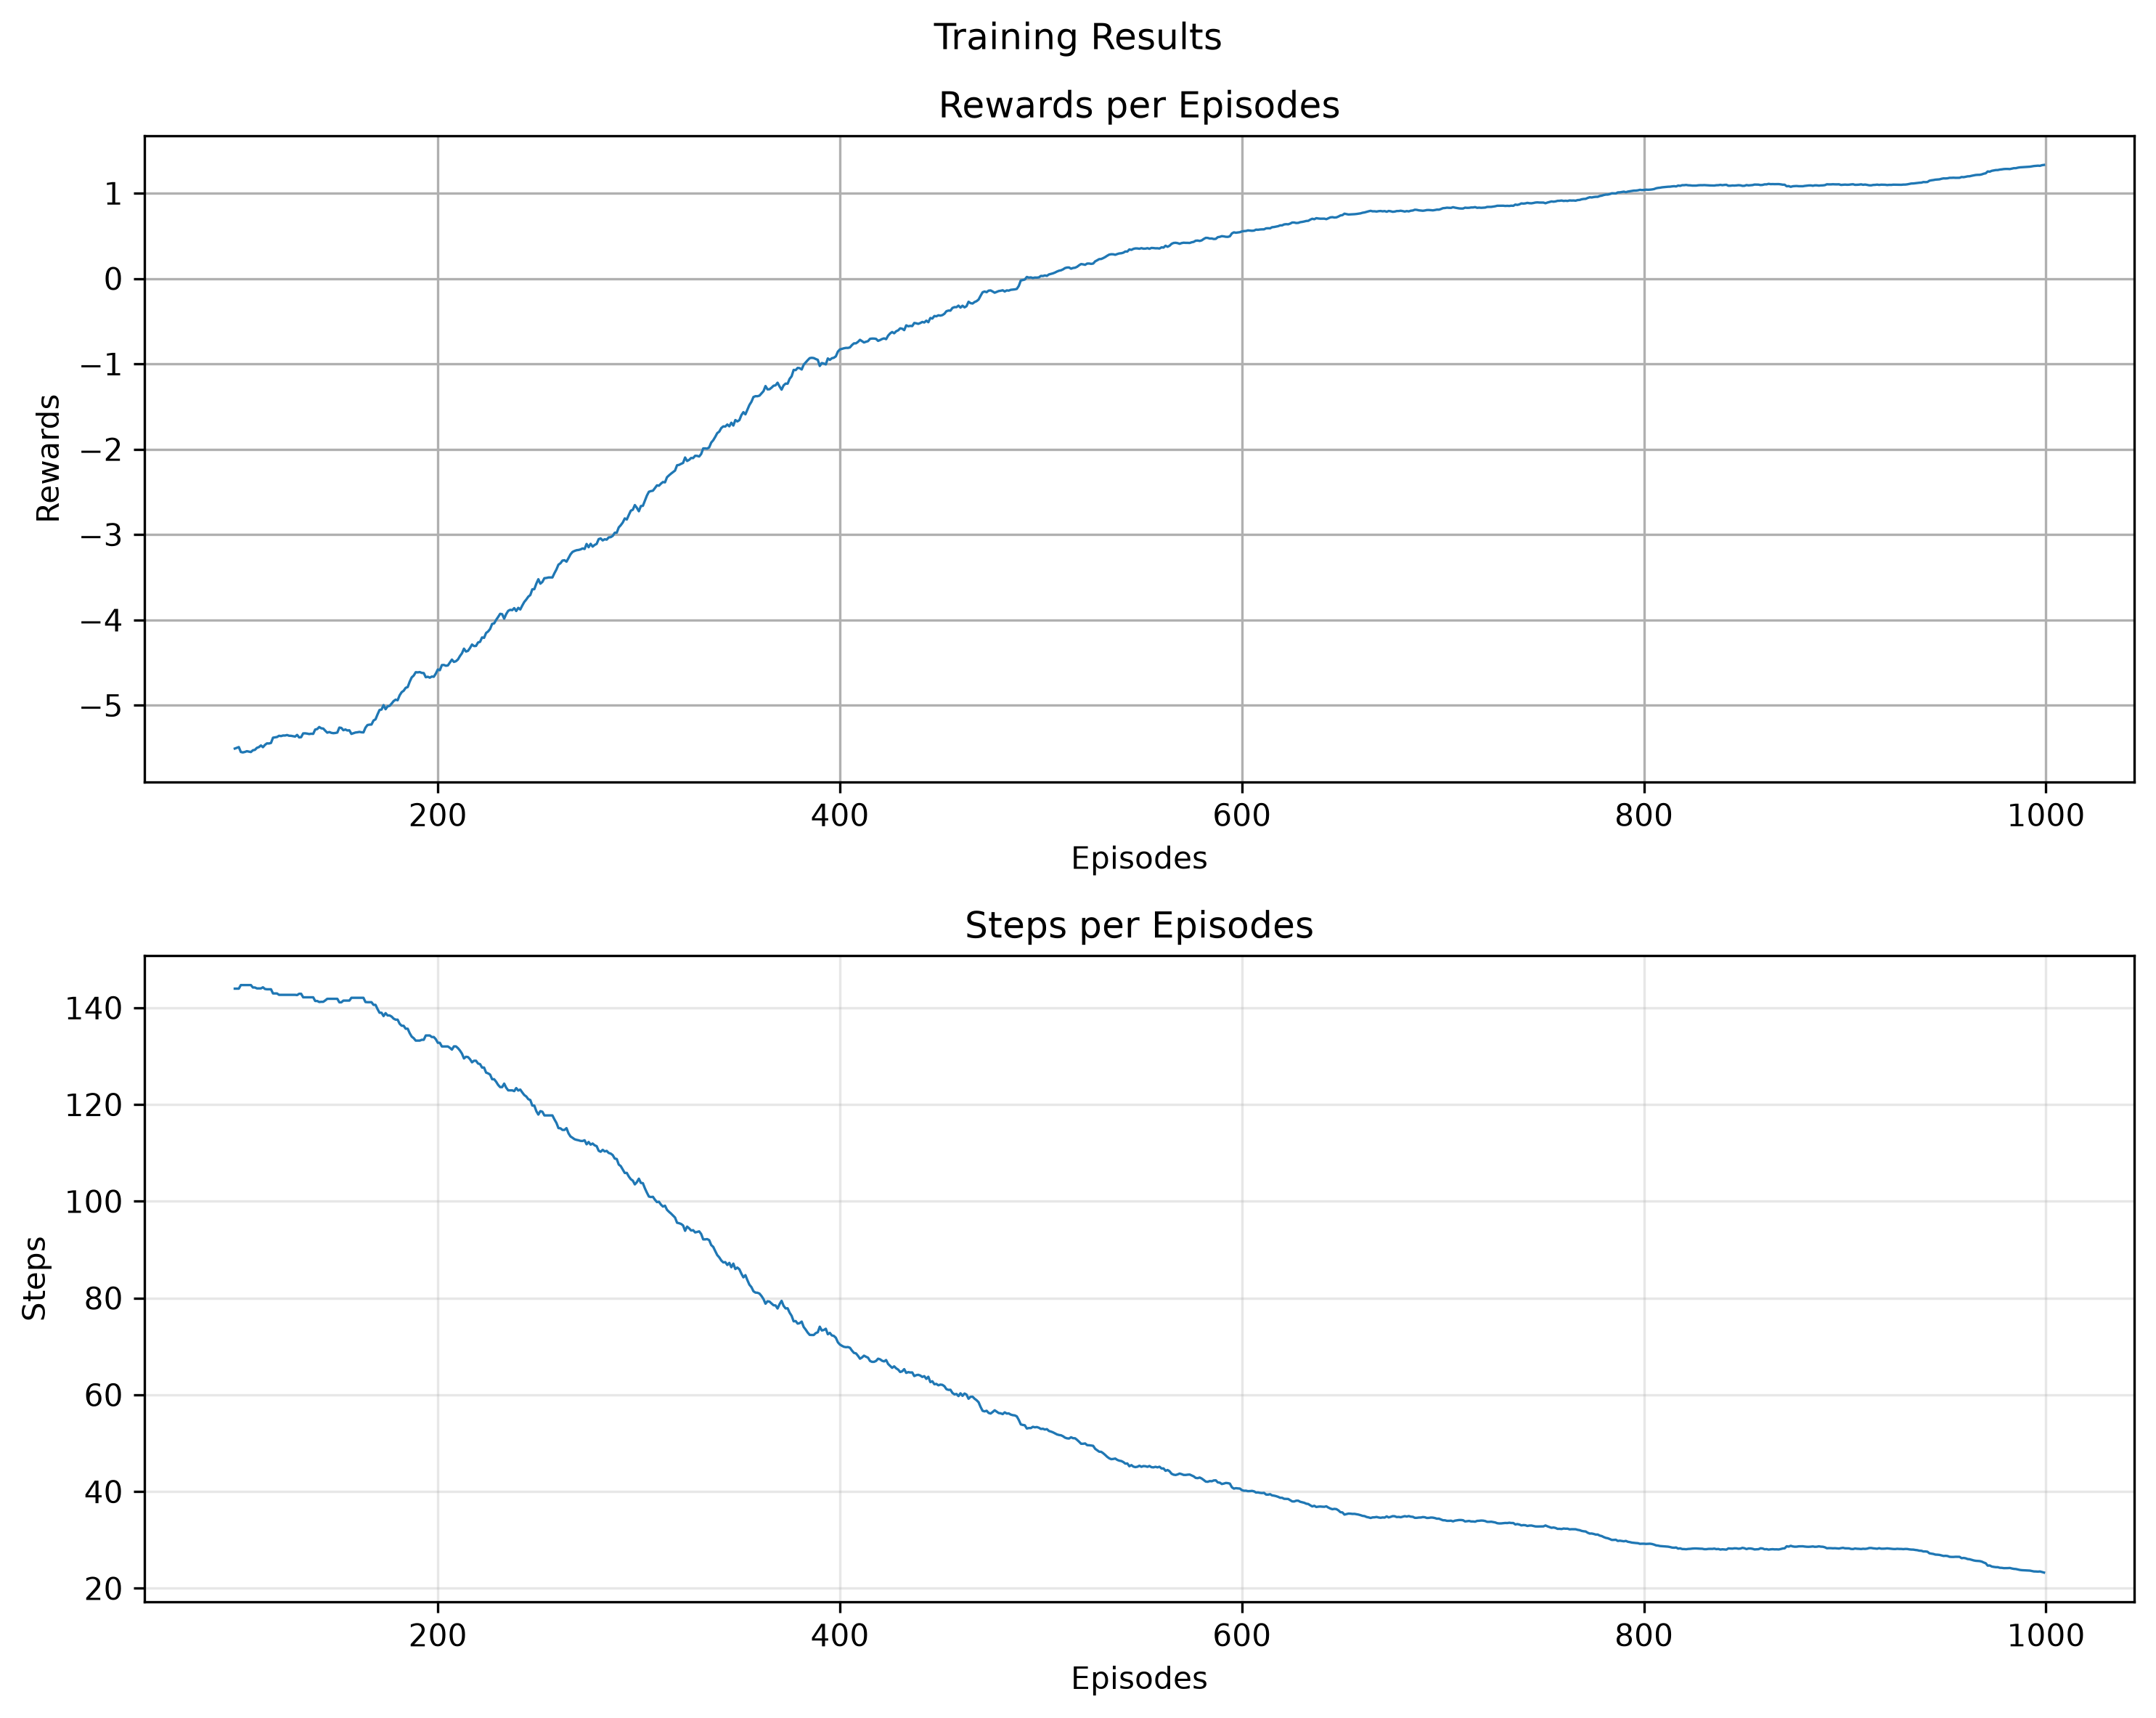
\includegraphics[scale=0.5]{./img/run_train.png}
        \caption{Training Result of 1000 episodes; top graph is reward per episode and bottom is steps per episode}
    \end{figure}
    \begin{figure}[!ht]
        \centering
        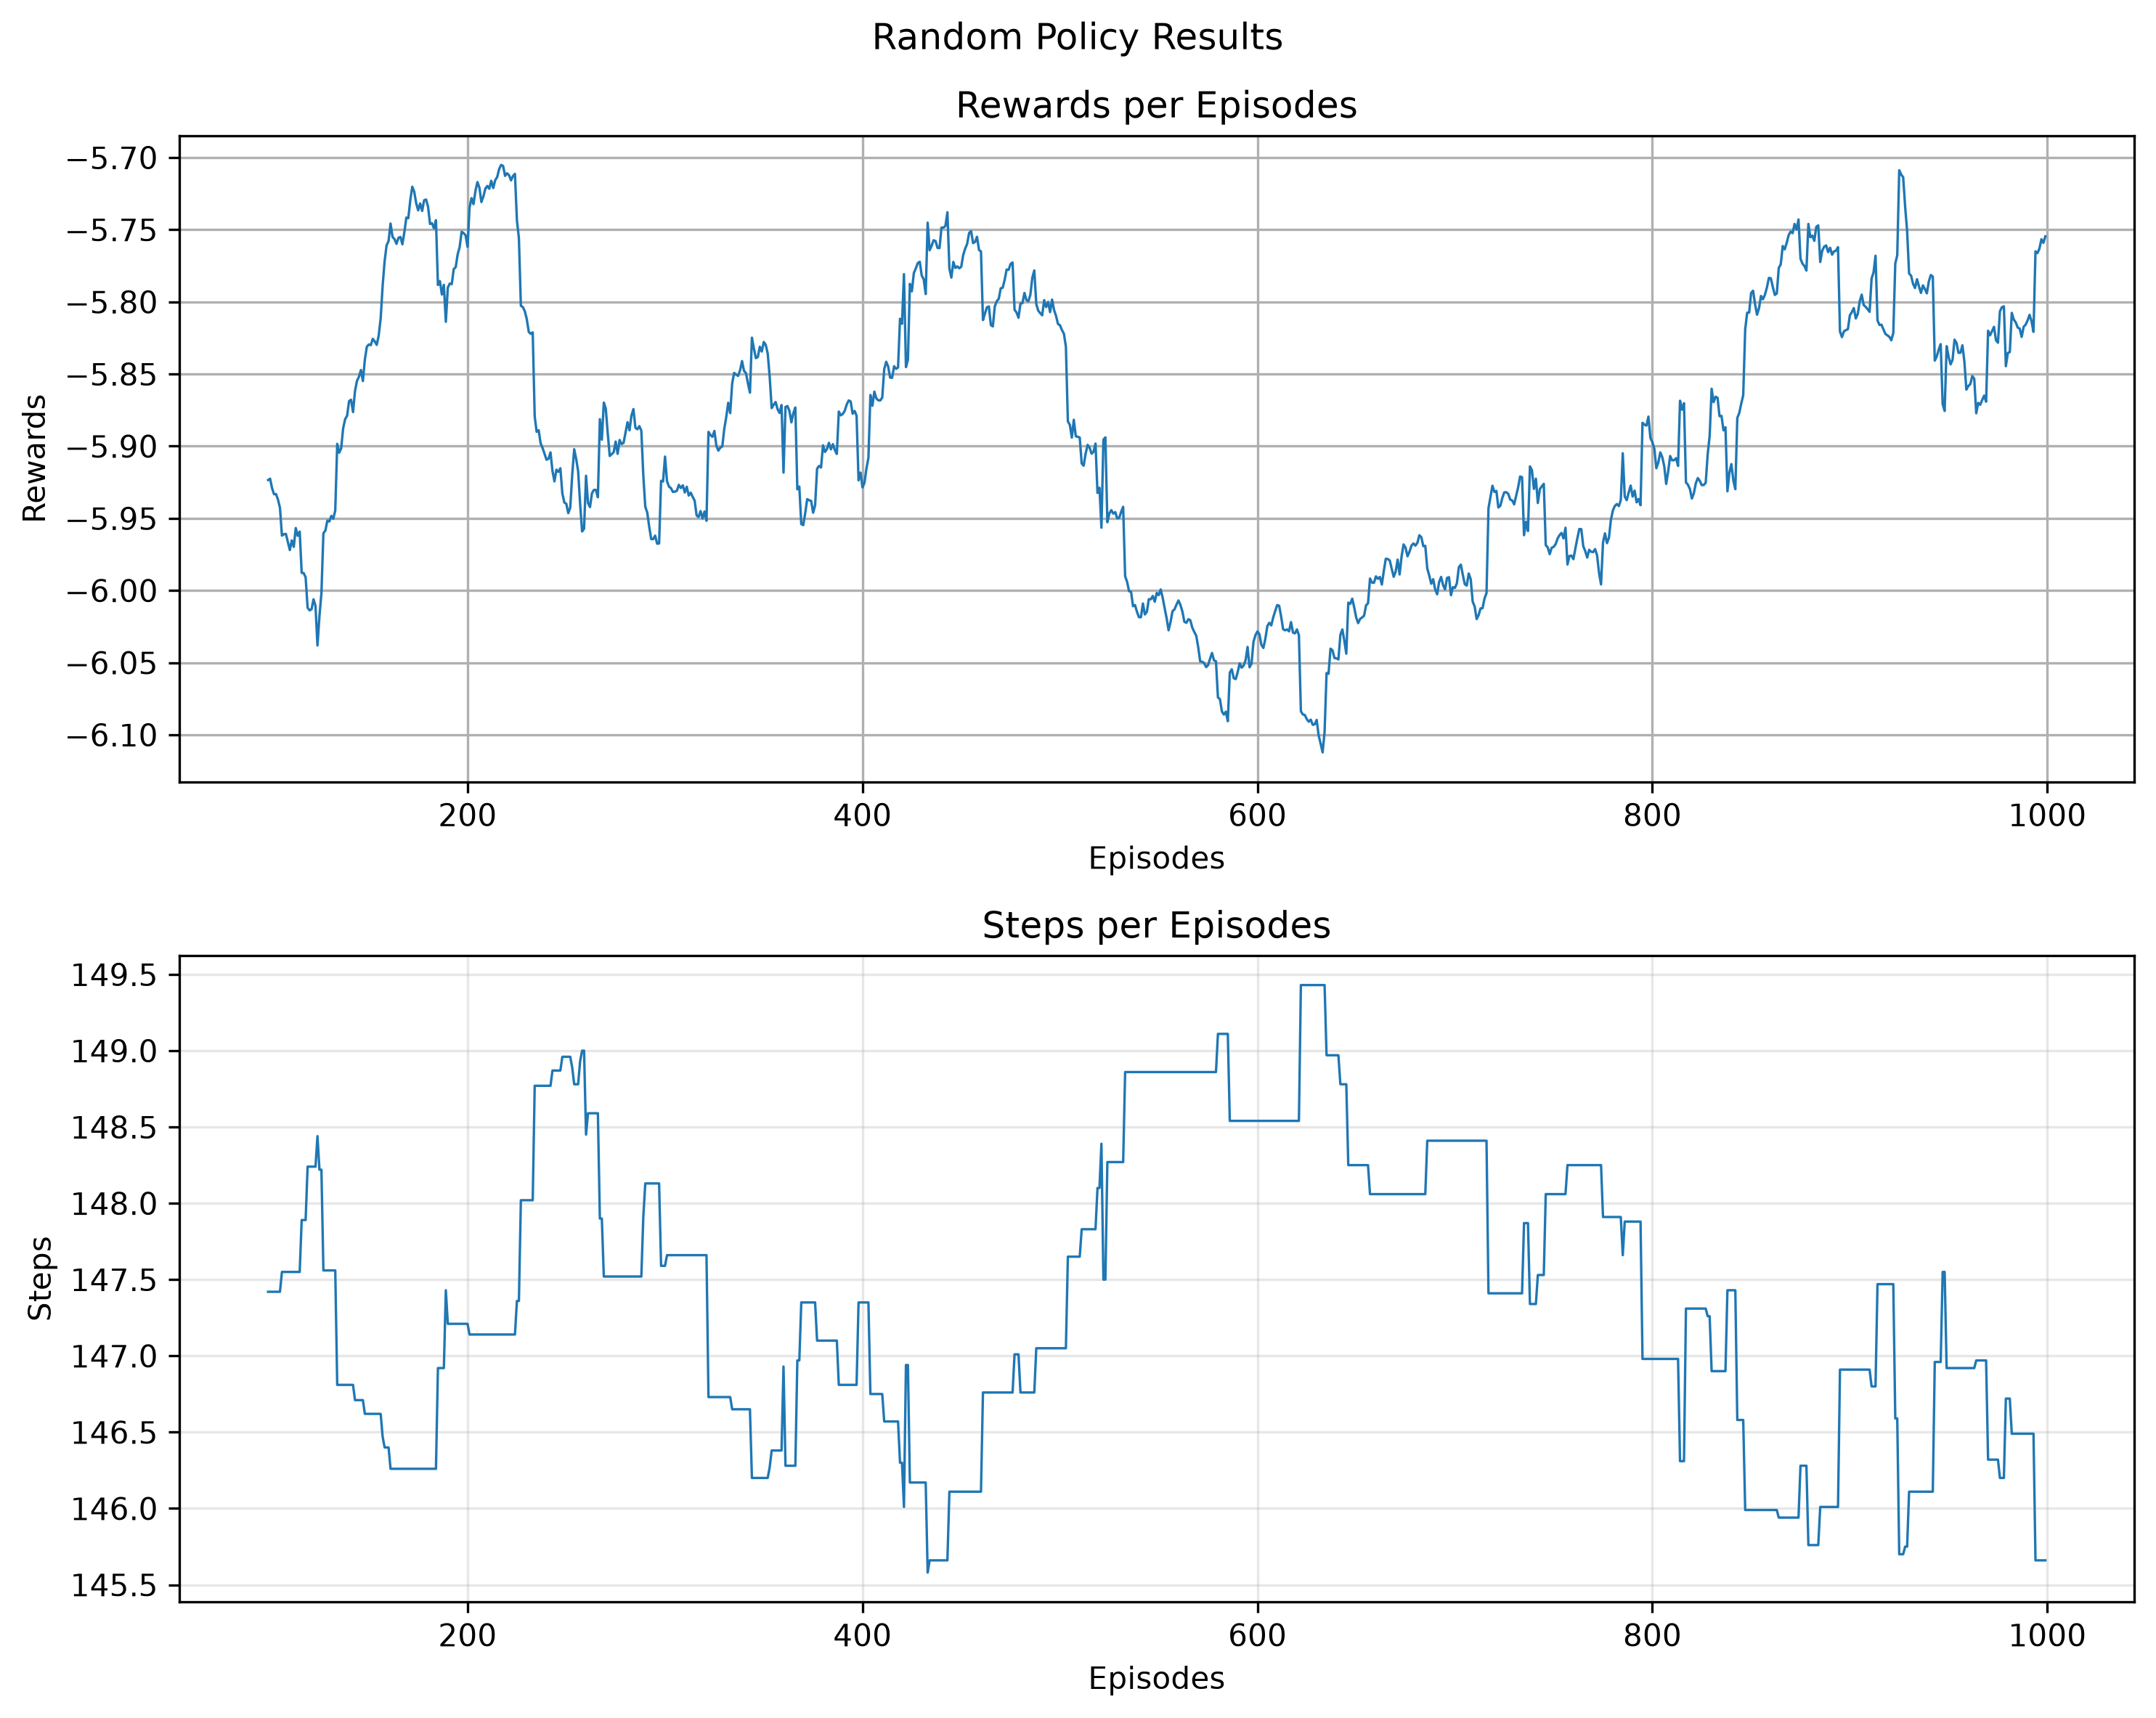
\includegraphics[scale=0.5]{./img/random_policy_results_eval.png}
        \caption{Result of implementing random policy for the agent and running it for 1000 episodes on the same grid}
    \end{figure}

    \FloatBarrier
    For figure 3, this displays how when implementing Q-learning with linear-decay, the agent improves over each episode.
    This can be seen by rewards increasing to 1.54 and the steps decreasing to 19 steps. Figure 4 represents the baseline of how the agent performs on the same grid for 1000 episodes.
    This shows through the training process, we are able to train an agent to discover the end goal of a grid.
    A demonstration video of the agent traversing the grid after training is in the zip file listed as \texttt{demonstration\_milestone3.mp4 }
    %-----------------------------------------%
    \section*{Next Steps}
    Current problems in the reinforcement agent involves the agent performing well in grids it was not trained on.
    This can be seen when a seed is not used inside the environment during evaluation, meaning a new grid is generated during each episode.
    The agent can sometimes find a path to the main objective, though it will not always be the shortest path.
    A goal for improving the model will be for the agent to achieve 90\% accuracy or greater during the evaluation loop with new grids being generated every episode. 
\end{document}
